\documentclass[a4paper,10pt]{article}
\usepackage{latexsym}
\usepackage[american]{babel}
\usepackage{lmodern}
\usepackage[utf8x]{inputenc}
\usepackage[T1]{fontenc}
\usepackage{longtable}
%\usepackage[dvips]{graphicx}
\usepackage{graphicx}

%\usepackage[pdftex]{hyperref}
\usepackage{hyperref}
\usepackage{amsmath}  % for equation environment
\usepackage{enumitem} % nolistsep to reduce list spacing

\usepackage{parskip} % no indentation in paragraphs

%opening
\title{Automated test generation for {\tt ctsa}}
\author{@hgfernan}
\frenchspacing

\pagestyle{myheadings}

\markboth{Automated test generation for {\tt ctsa}}
         {Automated test generation for {\tt ctsa}}

\addtolength{\hoffset}{-1,5cm}
\addtolength{\textwidth}{+3.5cm}

\addtolength{\voffset}{-1,2cm}
\addtolength{\marginparwidth}{-0,5cm}
\addtolength{\textheight}{+3.5cm}

% \linespread{1.5}


\begin{document}

\maketitle

\tableofcontents

\begin{abstract}
A routine for the automated test generation for the statistical
library {\tt ctsa} is outlined. It envolves the generation of
simple tasks of model fitting and prediction using {\tt ctsa},
compared with equivalent code in the Python libraries
{\tt pmdarima} and {\tt statsmodels}, and in the R library
{\tt forecast.}
\end{abstract}

\section{Motivation}
\label{sec:motiv}

{\em Why using a test database and automatic generation of
tests, instead of the handcrafted tests ?}

\section{Introduction}
\label{sec:intro}

{\em Overview of the project}

\section{Tables}
\label{sec:tables}

Since the automated test generation is based on a database, here
follows a description of the database to be used.

It has a mixed relational and document architecture: the main
tables follow a conventional relational structure, but the
parameters and test results are stored as JSON values. That's for
pragmatic reasons: the parameters and test results are varied and
have different structures. That could be easily mapped to a
relational database structure, but it would be too laborious and
cumbersome.

As such, test parameters and results will be stored as JSON
objects encoded as strings, and dealt with by classes specialized
in their content. That is:  an $ARIMA$ model will have three basic
parameters, while a $SARIMA$ model will have 7 basic parameters.
There will be a class for each one of the models, that will be
able to unpack and allow the use those JSON values.

\begin{figure}[h]
    \centering
    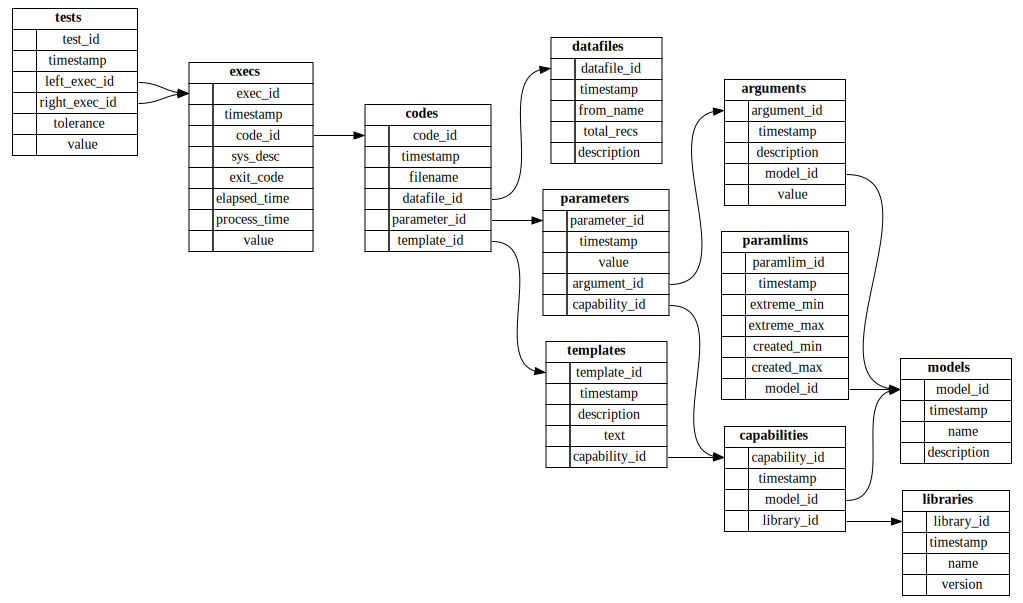
\includegraphics[scale=0.35]
        {../img/schema.jpg}
    \caption{Database used for automated test generation}
    \label{fig:schema}
\end{figure}

In a few words, the algorithm to generate tests follow this way:

\begin{enumerate}
    \item The table {\tt paramlims} (on the upper left corner of
        Figure \ref{fig:schema}) is used to select a sequence of
        parameters for each model, according to the limits present
        in the fields {\tt extreme\_min} and {\tt extreme\_max}.
        They are stored in the table {\tt params} to be detailed
        below.

        Not all parameters are generated, and the range of the
        parameters created up to the moment are saved in the
        fields {\tt created\_min} and {\tt created\_max}.

        The field {\tt timestamp} contains the last alteration
        of any or all values in the range {\tt created\_min} and
        {\tt created\_max} for its corresponding {\tt model};

    \item The list of data files available (stored in the folder
        {\tt data/}) are listed and each name is contained in the
        field {\tt filename} of the table {\tt datafiles}. In this
        table the date of each file inclusion is recorded in the
        field {\tt timestamp}. The field {\tt total\_recs} of the
        same table contain the number of records of each file.
        The field {\tt description} can be used to introduce
        details of the file: its origin, the transformations used
        to generate it, etc.

    \item \label{itm:codes}
        There are simple templates for each model, and they're
        used to generate a single file for each of the elements of
        the cartesian product between the allowed range of
        {\tt params} for each model, and the data files in
        {\tt datafiles}.

        This process is replicated for each of the languages in
        use (C, Python, and R) and their corresponding libraries
        {\tt ctsa}, {\tt pmdarima} and {\tt statsmodels}, and
        {\tt forecast}. Those results are stored in the table
        {\tt codes}, and only the programming language is stored
        there, as just a single library will be used for each
        case.

        After the testing {\em per se}, a fragment of the code
        stores in a CSV file the parameters, the calculated
        results and the elapsed and processing times, as well
        other information needed, as described in item
        \ref{itm:execs};

    \item \label{itm:execs}
        The codes generated are then run, as the resources in
        processing hardware and time allow for it.

        The execution results are stored in the table
        {\tt tables}, and they are retrieved from a CSV file
        that each execution generate, as described in the item
        \ref{itm:codes}.

        This table contains the field {\tt timestamp} that will
        inform when the execution was started. The field
        {\tt code\_id} refers to the source code that was used.
        The field {\tt sys\_desc} should contain a description
        of the hardware that was used to run the code, as precise
        as possible. Even though precision in the results is the
        main purpose of this suite of tests, a marginal point is
        the processing speed of each implementation. Of course,
        that comparison would be meaninful only if the execution
        scenarios of each benchmark participant were kept
        constant.

        The table also contains the fields {\tt elapsed\_time},
        that contains the clock time spent for the execution, and
        {\tt proc\_time} that contains the time spent using the
        processor or processors available in the hardware.

        Finally, the field {\tt value} is a JSON value encoded as
        a string that contain two data structures, named
        {\tt params}, where a copy of the model parameters is
        stored, and {\tt results}, where a copy of the numerical
        parameters is stored.

        There's some space for the results of a model -- for
        instance, the number of time steps forecasted --, but
        the intelligence to handle that variation will be kept in
        the class that handles each results;

    \item \label{itm:tests}
        Finally the table {\tt tests} holds what could be
        considered a test, actually a comparison between two
        executions, or fields in the table {\tt execs}.

        The field {\tt timestamp}, as usual, contains the
        information of the time when the comparison was started.
        The field {\tt left\_exec\_id} identifies the execution
        that will be compared against other execution, represented
        by the field {\tt right\_exec\_id}. Typically, it will be
        an execution of a program based upon {\tt ctsa} and
        another based upon one of its equivalent libraries using R
        or Python.

        And it is recommended that the comparisons are made only
        between two executions in the same hardware, described
        by {\tt sys\_desc}, as mentioned in the item
        \ref{itm:execs}.

        The comparison are executed against the value given in the
        field {\tt tolerance}. The relative deviation $d_{rel}$
        is calculated for each parameter as
        \begin{equation*}
            d_{rel} = \frac{ |p_{right} - p_{left}| }{p_{right}}
        \end{equation*}
        And a test passes when $d_{rel} \leq tolerance$; otherwise
        it fails.

        The field {\tt value} is a JSON value encoded as a
        structure, that contains two data structures, one named
        {\tt params}, where a copy of the model parameters is
        stored, and another named {\tt results}, that contains for
        each result a triplet with the numeric value of the result
        of the left test, the value of the result of the right
        test, and string ``{\tt pass}'' if the test passed, or
        ``{\tt fail}'' if the test failed.

\end{enumerate}

\section{Software design}
\label{sec:design}

{\em High level specification of the softwares and their use.}

\section{Examples by hand}
\label{sec:by_hand}

{\em Worked examples of the database and software use.}

\section{Implementation}
\label{sec:impl}

{\em A shiplog reporting details of the system development, and
possible deviations from the specification in the section
\nameref{sec:design}}.

\end{document}
